%\documentclass[12pt,a4paper]{report}


%&pdflatex
\pdfobjcompresslevel 0 % Ligne souvent nécessaire pour la validité du PDF généré
\documentclass[french,12pt,a4paper]{report}
\usepackage[top=1.5cm,bottom=2cm,left=2.5cm,right=2.5cm,includehead]{geometry}
\usepackage[T1]{fontenc}% pour la sortie
\usepackage[utf8]{inputenc} % pour l'entrée
\usepackage{graphicx}
\usepackage{setspace}

% #region Packages
\renewcommand{\rmdefault}{phv}	% Utilise la police Arial pour le texte
\usepackage[T1]{fontenc}		% Encodage de la police pour une meilleure gestion des caractères spéciaux
\usepackage[utf8]{inputenc}		% Encodage UTF-8 pour permettre l'utilisation de caractères non-ASCII
\usepackage{lmodern}			% Utilise une version améliorée des polices LaTeX standard
\usepackage{graphicx}			% Permet d'insérer des images dans le document
\usepackage{multicol}			% Gère le texte en colonnes multiples
\usepackage{lipsum}				% Génère du texte factice (Lorem Ipsum)
\usepackage{float}				% Améliore le placement des objets flottants (comme les figures et tableaux)
\usepackage{vwcol}				% Permet de créer des colonnes avec des largeurs variables
\usepackage{geometry}			% Permet de définir les marges et la mise en page
\usepackage{caption}			% Personnalise les légendes des figures et tableaux
\usepackage{framed}				% Encadre des portions de texte
\usepackage{pdflscape}			% Permet d'inclure des pages en mode paysage dans un PDF
\usepackage{eurosym}			% Ajoute le symbole de l'euro (€)
\usepackage{xcolor}				% Gestion avancée des couleurs dans le document
\usepackage{amsmath,amssymb}	% Fournit des symboles et des outils avancés pour les mathématiques
\usepackage{hyperref}			% Ajoute des liens hypertextes cliquables dans le PDF
\usepackage{setspace}			% Gère l'espacement entre les lignes

% #endregion

% #region Déclaration des couleurs
\definecolor{tabblue}{RGB}{31,119,180}
\definecolor{taborange}{RGB}{255,127,14}
\definecolor{tabgreen}{RGB}{44,160,44}
\definecolor{tabred}{RGB}{214,39,40}
\definecolor{tabpurple}{RGB}{148,103,189}
\definecolor{tabbrown}{RGB}{140,86,75}
\definecolor{tabpink}{RGB}{227,119,194}
\definecolor{tabgray}{RGB}{127,127,127}
\definecolor{tabolive}{RGB}{188,189,34}
\definecolor{tabcyan}{RGB}{23,190,207}
\definecolor{rosePW}{RGB}{219,164,207}
\definecolor{orangeNW}{RGB}{245,121,0}
% #endregion

\geometry{a4paper, left=25mm, right=25mm, top=25mm, bottom=25mm}
\DeclareCaptionType{annexe}


% Espacement entre les lignes
\onehalfspacing



\usepackage{hyperref}
\hypersetup{
    colorlinks=true,
    linkcolor=black,
    filecolor=black,
    urlcolor=black,
    % bookmarks=true,
    bookmarksopen=true,
    bookmarksopenlevel=2,
    pdftitle={Manuscrit de thèse de Maxime Guillot},
    pdfauthor={Maxime Guillot},
}

% Set up section numbering
\setcounter{secnumdepth}{4}


\usepackage{titlesec}
\titleformat{\paragraph}
{\normalfont\normalsize\bfseries}{\theparagraph}{1em}{}
\titlespacing*{\paragraph}
{0pt}{3.25ex plus 1ex minus .2ex}{1.5ex plus .2ex}


% #region Déclaration des "Mets une source"
\usepackage{etoolbox}
\BeforeBeginEnvironment{metsUneSource}{\colorlet{oldcolor}{.}}
\AfterEndEnvironment{metsUneSource}{\color{oldcolor}}

\newenvironment{metsUneSource}
{\begin{framed}\color{red}}
{\end{framed}}
% #endregion

% % Création de l'environnement 'spaced' avec interligne doublé
% \newenvironment{spaced}
%     {\begin{spacing}{2}} % Interligne doublé
%     {\end{spacing}}

\newcommand{\HRule}{\rule{\linewidth}{0.5mm}} % Une ligne horizontale de la largeur de la page

\begin{document}

% ----------------------------- %
%          Document principal    %
% ----------------------------- %

% Inclusion de la première de couverture
\begin{titlepage}
    \begin{center}
        % Logo de l'université (facultatif)
        
\includegraphics[width=0.2\textwidth]{figures/universite_de_bordeaux.pdf} \\
        \vspace{1cm}

        % Nom de l'université
        \textsc{\Large Université de [Nom de ton université]}\\[0.5cm]

        % Faculté ou département
        \textsc{\Large [Nom de la faculté ou du département]}\\[1.5cm]
\begin{spacing}{2}
     % Titre de la thèse
     \HRule \\[0.4cm]
     { \huge \bfseries Référence de tension en technologie CMOS désensibilisée au débit de dose en environnement radiatif sévère : un verrou technologique pour le démantèlement des centrales nucléaires}\\[0.4cm]
     \HRule \\[1.5cm]
\end{spacing}
       

        % Sous-titre (si applicable)
        { \large Voltage reference in CMOS technology desensitized to the dose rate in a harsh radiation environment for the dismantling of nuclear power plants}\\[1.5cm]

        % Auteur
        \textsc{\Large Présenté par :}\\[0.4cm]
        \textsc{\large Maxime [Ton nom de famille]}\\[2cm]

        % Diplôme
        \textsc{\Large En vue de l'obtention du diplôme de [Nom du diplôme]}\\[1cm]

        \begin{flushleft}
            % Jury
            \textsc{Jury :}\\[0.4cm]
            \begin{tabular}{ll}
                Prénom NOM & Fonction \\
                Prénom NOM & Fonction \\
                Prénom NOM & Fonction \\
                Prénom NOM & Fonction \\
                Prénom NOM & Fonction \\
            \end{tabular}
        \end{flushleft}
 
    \end{center}
\end{titlepage}

%%&pdflatex
\pdfobjcompresslevel 0 % Ligne souvent nécessaire pour la validité du PDF généré
\documentclass[french,12pt,a4paper]{report}
\usepackage[top=1.5cm,bottom=2cm,left=2.5cm,right=2.5cm,includehead]{geometry}
\usepackage[T1]{fontenc}% pour la sortie
\usepackage[utf8]{inputenc} % pour l'entrée
\usepackage{graphicx}
\usepackage{setspace}

\begin{document}
\pagestyle{empty}
% Les logos en tête, ici une seule image incluse
%\includegraphics[scale=1, height=1.7cm]{images/logo0.png}
%\hfill
%\includegraphics[scale=1, height=1.7cm]{images/logo1.png}
%\hfill

\includegraphics[scale=1, height=1.7cm]{images/brdx.pdf}
\hfill

\includegraphics[scale=1, height=1.7cm]{images/brdx.pdf}
\hfill
%\includegraphics[scale=1, height=1.7cm]{images/logo4.jpg}
\begin{center}
\doublespacing
\begin{Large}

THÈSE PRÉSENTÉE\\ POUR OBTENIR LE GRADE DE \\
{\LARGE \textbf{DOCTEUR\\DE L'UNIVERSITÉ DE BORDEAUX} } \\
\vspace{0.55cm}
ECOLE DOCTORALE SCIENCES ET ENVIRONNEMENTS\\
{\normalsize ECOLOGIE ÉVOLUTIVE, FONCTIONNELLE ET DES COMMUNAUTÉS} \\
\vspace{0.55cm}
Par \textbf{Harry COVERT} \\
\vspace{0.55cm}
{\Large Titre de la thèse décrivant avec les mots clés nécessaires la thématique précise étudiée et les travaux effectuées}
\end{Large}
\vspace{0.55cm}
\begin{normalsize}
\begin{singlespace}
Sous la direction de : \textbf{Jane DOE}\\
Co-directrice : \textbf{Simone UNTEL}
\end{singlespace}
\end{normalsize}
\end{center}
\vfill
{\large Soutenue le 25 décembre 2019 }\\
\vfill
Membres du jury :
\begin{table}[b]
\centering
\makebox[\textwidth]{%
\begin{tabular}{lllr}
Mme. Aude ALPHA       & Directrice de Recherche & Université & Rapporteur  \\
M. Bernard BETA       & Directeur de Recherche  & Université & Rapporteur  \\
M. Georges GAMMA      & Directeur de Recherche  & Université & Président   \\
Mme. Dominique DELTA  & Chargée de Recherche    & Université & Examinatrice\\
M. Eric EPSILON       & Ingénieur de Recherche  & Université & Examinateur \\
Mme. Jane DOE         & Directrice de Recherche & Université & Directrice  \\
Mme. Simone UNTEL     & Ingénieure de Recherche & Université & Invitée     \\
\end{tabular}
}
\end{table}
\end{document}




% % ----------------------------- %
% %          Préface               %
% % ----------------------------- %
% \chapter*{Préface}
% \addcontentsline{toc}{chapter}{Préface}  % Ajout au sommaire
% % Écrire la préface ici
%----------------------------- %
%          Remerciement               %
% ----------------------------- %
\chapter*{Remerciements}
\addcontentsline{toc}{chapter}{Remerciements}  % Ajout au sommaire
% Écrire la préface ici

%Mon amoureux, Antoine D 
%Mon bébé, Marie P


% ----------------------------- %
%        Table des matières      %
% ----------------------------- %
\tableofcontents
\newpage

% ----------------------------- %
%      Chapitre d'introduction   %
% ----------------------------- %
\chapter*{Introduction}
% Écrire l'introduction ici
 

% ----------------------------- %
%        Chapitre 1              %
% ----------------------------- %
\chapter{Effet des radiations sur les composants électroniques}
% Inclure un fichier séparé pour chaque chapitre
% \input{chapitre1}

metsUneSource


\lipsum[1-2]

\begin{metsUneSource}
\lipsum[3]
\end{metsUneSource}

\textit{dcnduvbdvbdbvdiubvk}

% ----------------------------- %
%        Chapitre 2              %
% ----------------------------- %
% Inclure un fichier séparé pour chaque chapitre
% \input{chapitre2}
\chapter{Design d'un circuit intégré pour les conditions extrêmes}
%spec aifira
%supression diode antenna

\section{Diodes \textit{"gate antenna"} , Origine – Impact – Suppression}

Comme expliqué dans la partie \textcolor{red}{tutu}, les jonctions PN, lorsque qu'elles sont soumisent à des radiations, sont des sources de courants parasites qui peuvent perturber le fonctionnement du circuit. Une manière de limiter ces courants est de limiter le nombre de jonction PN dans le circuit. Malheureusement, certaines jonctions PN sont imposée par le fondeur, c'est notament le cades des diodes dite de \textit{gate-antenna}.

\subsection{Origine}
\begin{metsUneSource}
  Le processus de fabrication des circuits intégrés contient des étapes de polissages après la dépose et lithographie de chaque niveau de métal.
\end{metsUneSource}


\begin{metsUneSource}
  Les étapes de polissages sont des étapes à risque car en tournant, le matériel de polissage va arracher des charges électriques au circuit qui va alors être soumis à des tension et champs électriques plus ou moins intense.
\end{metsUneSource}
Les étapes de gravure au plasma des différents niveaux de métaux, sont susceptibles de charger électriquement les pistes du circuit.

\begin{metsUneSource}
Thin gate oxide damage due to plasma processing
\end{metsUneSource}

Ce phénomène est connu sous le nom d'\textit{antenna-effect} soit "effet antenne". Les tensions et champs électriques généré par l'effet antenne présentent un risque de décharge électrique à travers le circuit ce qui peut endommager le circuit de manière irréversible lors de sa construction.

\begin{metsUneSource}
Source 
\end{metsUneSource}


Une méthode régulièrement utilisée pour minimiser les risques de destruction du circuit par l'\textit{antenna-effect} consiste à mettre des diodes qui permettent d’évacuer les charges électrique dans un chemin guidé, les empêchant ainsi de passer par le circuit, le détériorant.
\begin{metsUneSource}
  Thin gate oxide damage due to plasma processing
\end{metsUneSource}

\begin{metsUneSource}
Parles des grilles

Calcul diode \textit{gate-antenna} cas FDSOI
\end{metsUneSource}

Les erreurs de \textit{gate-antenna} sont détectés par le DRC qui fait le calcul basé sur l'équation \ref*{eq:metalX2000}.

\begin{equation}
  S_{Metal_{X}} <2000 \times S_{R_{X} on insulator}+50 \times S_{R_X bulk}
  \label{eq:metalX2000}
\end{equation}

Cette équation indique que la surface d'un metal donné  $S_{Metal_{X}}$ correspondant à un noeuds éléctrique ne doit pas dépasser 2000 fois la valeur de la sommes des surfaces de la couche active SOI $S_{R_{X} on insulator}$ et 50 fois celles surface des couches actives dans le substrat $S_{R_X bulk}$.

\subsection{Couche active $R_{X}$ et erreurs de \textit{gate-antenna}}
La couche active $R_{X}$ est la couche qui est déssiné lors du layout du circuit et qui permet de définir les zones "actives" du circuit. Ces zones correspondent aux emplacements des transistors et aux differents contact entre le niveau de métal le plus bas $M_1$ et le silicium. Elles indique au fondeur de doper le silicium à de plus forte concentration en trous ou en electron suivant si le silicium est normalement N ou P. Ceci permet d'eliminer les diodes Shotckley entre les métaux et le silicium. Ce processus est résumé brièvement dans la figure %\ref*{fig:process fdsoi}.

\begin{figure}[H]
  \centering
  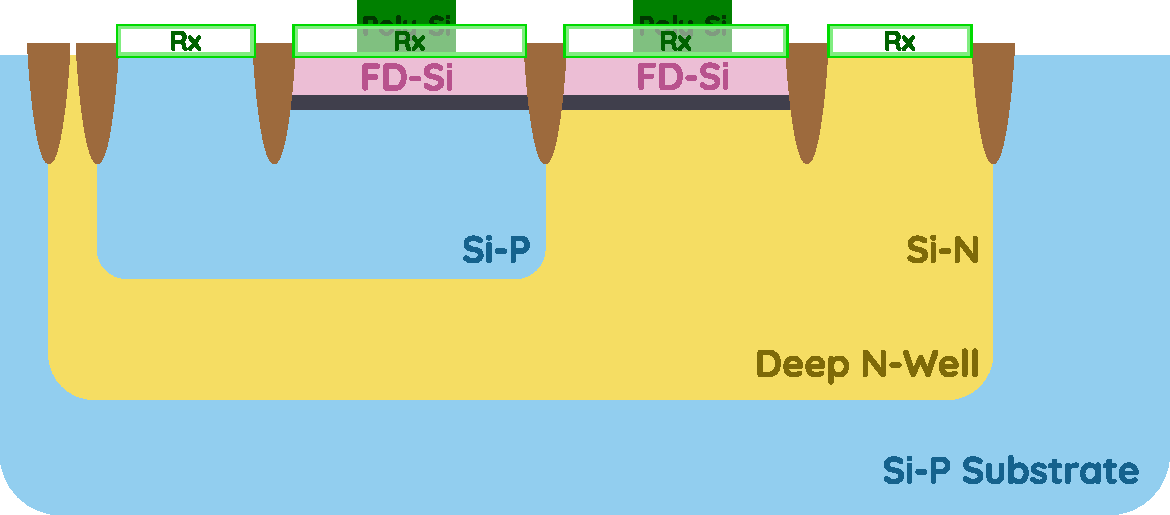
\includegraphics[width=0.7\textwidth]{figures/FabSOI-MiddleEND-2.pdf}
  \caption{Processus de fabrication d'un circuit en technologie FD-SOI: les isolants, les puits et les grilles sont déjà créés}
  \label{fig:process fdsoi 2}
\end{figure}

\begin{figure}[H]
  \centering
  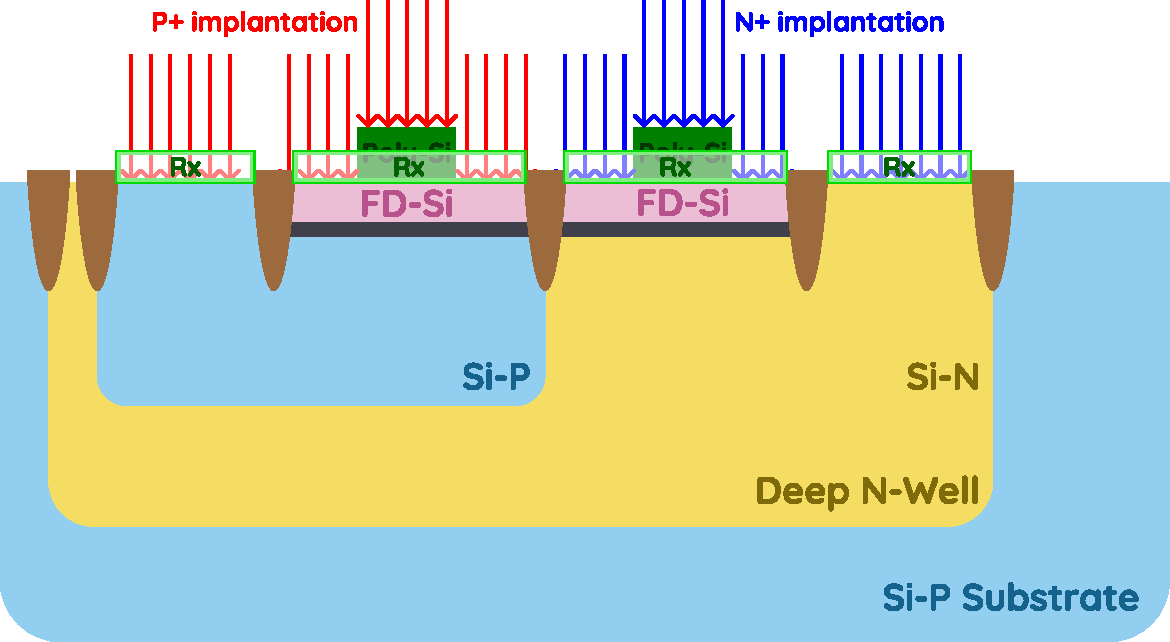
\includegraphics[width=0.7\textwidth]{figures/FabSOI-MiddleEND-3.5.pdf}
  \caption{Implatation des dopants de surface au niveau des zones actives, la couche $R_X$ n'est pas physique mais donne juste une indication. Les dimensions réelles ne permettent pas de doper d'un coté puis de l'autre de la grille.}
  \label{fig:process fdsoi 3}
\end{figure}


\begin{figure}[H]
  \centering
  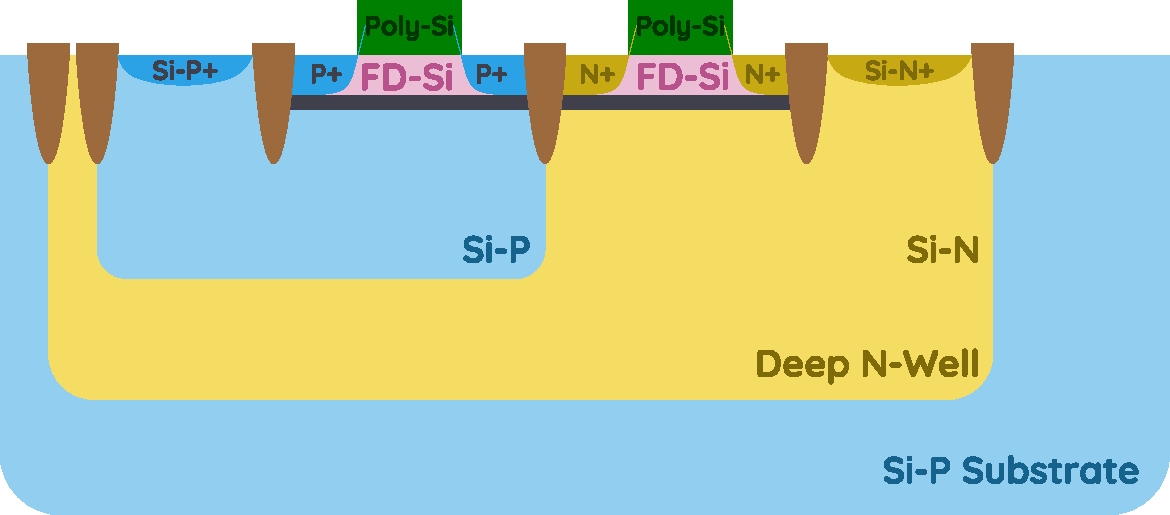
\includegraphics[width=0.7\textwidth]{figures/FabSOI-MiddleEND-4.pdf}
  \caption{La surface du silicium est plus dopée que dans la profondeur du substrat, le Poly Silicium, masquant l'implantation au niveau du canal, permet de concerver un canal "\textit{Fully Depleted}"}
  \label{fig:process fdsoi 4}
\end{figure}

\subsection{Impact}
En règle générale, les diodes \textit{gate-antenna} ont un impact réduit sur les performances des circuits, augmentant simplement les capacité parasites des (normalement déjà élevé car beaucoup de métal) nœuds auxquels elles sont connectées. Dans le cadre d’un circuit destiné aux environnements radiatifs, les diodes \textit{gate-antenna} ont un impact bien plus important. En effet, au même titre que les autres jonctions PN, les diodes \textit{gate-antenna}, soumises à des radiations vont générer des courants parasites. De plus, contrairement aux diodes des \textit{Back-Gates} dont les courants parasites peuvent éventuellement être évacués par les alimentations \textcolor{red}{(cf. §III.A)}, il peut être nécessaire de mettre des diodes \textit{gate-antenna} n’importe où et notamment à des parties du circuit qui ne peuvent pas être régulé par une alimentions qui imposerait sa tension, compensant le courant parasite.
\begin{metsUneSource}
  Schéma Vref avec diode et du courant
\end{metsUneSource}

Dans cette étude, les règles de dessin nous imposent de mettre une diode \textit{gate-antenna} en sortie du circuit. En respectant cette règle, on s’assure d’avoir des performances médiocres face aux radiations, le courants parasite étant directement envoyé dans le circuit, perturbant sont point de fonctionnement et dans la sortie, modifiant la valeur de la référence de tension. Déroger à cette règle, c’est prendre le risque d’une destruction du circuit lors de sa fabrication.

\subsection{Suppression}
Différentes techniques existent pour se passer des diodes \textit{gate-antenna} mais sans qu’aucune ne soit parfaite :
\paragraph{Reduction du rapport des surfaces métal/grille}
Les diodes \textit{gate-antenna} n’étant nécessaire que dans le cas où la surface de métal connecté à une grille de transistor est trop importante, la première idée est de réduire au minimum la surface de métal connecté. L’inconvenant de cette technique est qu’elle élimine la possibilité de mettre du mesh. En effet le mesh consiste à mettre de grande quantité de métaux sur le circuit dans le but de former des capacités qui viendront lisser les tensions du circuit et limiter les risques d’oscillations et perturbations.

\begin{metsUneSource}
Photo plot
\end{metsUneSource}

Aussi, comme ce le cas dans notre étude, la surface des plots permettant l’accès au circuit par l’extérieur, en Wire-Bonding ou sous pointes, peut déjà dépasser la surface maximale accepté par les règles de dessin pour ne pas nécessiter de diode \textit{gate-antenna}. La taille et la densité du plot ne pouvant pas être diminuer sous peine de ne pas pouvoir connecter le circuit.

A l'inverse, il est également possible de diminuer le rapport des surfaces métal/grille en augmentant la taille des grilles, soit en utilisant des transistors plus gros, ce qui demande un redimensionnement du circuit, soit en ajoutant des \textit{dummies}, qui est généralement obligatoire pour l'appariement des transistors.
Dans le cas de l'ajout de \textit{dummies}, comme expliqué dans la partie : \textcolor{red}{III.B.1)} Motivations, la technologie 28nm FDSOI permet d'ajouter des \textit{dummies} sans augmenter la taille finale des diodes \textit{gate-antenna}.

\begin{metsUneSource}
Explication rx
\end{metsUneSource}


\paragraph{Bridging}
Le calcul des surfaces métalliques qui entre en compte dans le calcul des surfaces des diodes \textit{gate-antenna} est fait pour chaque couche de métal, une gestion judicieuse des niveaux de métaux permet de modifier les surfaces entrant en jeu afin de se passer des diodes. 
En effet, la technique dite de bridging permet de réduire la surface de métal connecté électriquement à la grille de transistor concernée, elle consiste à relier deux morceaux de piste d'un métal d'un niveau \textbf{n} par le métal de niveau \textbf{n+1} comme présenté en 

\begin{metsUneSource}
  Fig. 1 .Source bridging
\end{metsUneSource}

\begin{figure}[H]
  \centering
  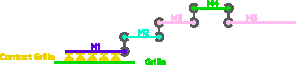
\includegraphics[width=0.7\textwidth,keepaspectratio]{figures/BridgingBon.pdf}
  \caption{Exemple de bridging entre deux pistes de métal, le métal M3 est bridgé par le métal M4.}
  \label{fig:Bridging}
\end{figure}

Ainsi, lors de la gravure du métal de niveau \textbf{n}, sa surface est limitée, les problèmes de \textit{gate-antenna} disparaissent.
La taille des plots de connexion, comme dans le paragraphe précèdent, peut tout de même venir annuler les effets du bridging.

\begin{figure}[H]
  \centering
  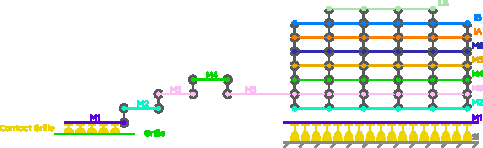
\includegraphics[width=0.7\textwidth,,keepaspectratio]{figures/BridgingPAD.pdf}
  \caption{Bridging de M3 par M4 connecté à un plot.}
  \label{fig:BridgingPlot}
\end{figure}


\paragraph{Dérogation auprès du fondeur}
La solution ultime, quand aucune autre solution n’a permis de se passer des diodes \textit{gate-antenna} est de demander, au fondeur, une dérogation sur l’erreur de dessin impliquant les diodes \textit{gate-antenna}. Cette solution est très risquée car le fondeur se libère de toute responsabilité quant à la bonne fabrication du circuit, qu’il est très difficile de prouver que le circuit ait été détruit par des ESD et qu’il serait osé de proposer une technique si hasardeuse sur une production à grande échelle, le nombre de circuit défectueux dès la sortie d’usine serait alors trop nombreux.

\subsection{Drainage des courants parasites}
\label{sec:drainage}

Afin de réduire l'impact des courants générés par les jonctions PN des \textit{Back-Gates}, un solution est de drainer ces courants vers l'alimentation et la masse du circuit qui sont théoriquement des points de tension fixe. Cette solution est présentée dans la figure \textcolor{red}{ ref*{fig:drainage}.}

\begin{metsUneSource}
fig drainage
\end{metsUneSource}
\subsection{Technologie 28nm FDSOI}

La fabrication de deux circuits s'est effectuée sur la technologie 28nm FDSOI de chez  \textit{ST Microelectronics}. Cette technologie est une technologie de pointe qui permet de fabriquer des circuits intégrés performants et qui, de par la présence de sa Back-Gate permet une grande flexibilité de fonctionnement. Aussi, la technologie FDSOI est connue pour sa robustesse aux radiations.



La Figure \ref{fig:coupeNMOS} est une vue en coupe d'un transistor LVT-NMOS, ou transistor NMOS à faible tension de seuil (Low-$V_{th}$-NMOS), fabriqué en technologie 28nm FD-SOI. En technologie FD-SOI, les transistors sont construits sur un isolant, ce qui permet au canal d’être entièrement déplété. Le silicium sous la couche d’isolation est dopé de type N dans le cas du LVT-NMOS et est appelé la grille arrière (back-gate).


\begin{figure}
    \centering
    \includegraphics[width=0.8\linewidth]{../Conf/ICECS2024/ICECS_Voltage_Reference/figures/LVT-NMOS.pdf}
    \caption{vue en coupe d’un transistor NMOS en technologie FD-SOI 28 nm \cite{cathelin_fully_2017}.}
    \label{fig:coupeNMOS}
\end{figure}

\subsubsection{Influence de la Back-Gate} 
La technologie FDSOI est une technologie qui permet de contrôler la tension de seuil des transistors en agissant sur la tension de la Back-Gate.  En effet, en appliquant une tension sur la Back-Gate, on crée un champ électrique qui va modifier la concentration de porteurs dans le canal du transistor. Cette modification de concentration de porteurs va modifier la tension de seuil du transistor. La techn FDSOI permet donc un controle fin de la tension de seuil et de la performance des transistors au travers d'une tension.

\begin{figure}
    \centering
    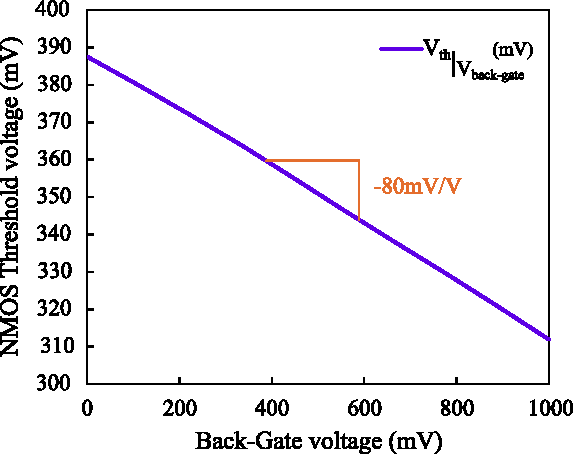
\includegraphics[width=0.7\textwidth]{../Conf/ICECS2024/ICECS_Voltage_Reference/figures/Vt(Vbb).pdf}
    \caption{Evolution de la tension de seuil en fonction de la tension de la Back-Gate}
    \label{fig:Vt(Vbb)}
\end{figure}

La tensions de seuil variant linéairement avec la tension de la Back-Gate, il est possible de determiner l'équation de la tension de seuil en fonction de la tension de la Back-Gate. Cette équation est donnée par l'équation \ref{eq:Vt(Vbb)}.

\begin{equation}
    V_{th}(T) = \beta V_{BB} + V_{th_0}\hspace*{0.3cm}(V)
    \label{eq:Vt(Vbb)}
\end{equation}
Avec:

\begin{itemize}
    \item $\beta$ : la sensibilité de la tension de seuil à la tension de la Back-Gate en $mV/V$, ici: $\beta=80mV/V$.
    \item $V_{BB}$ : la tension de la Back-Gate.
\end{itemize}


% ----------------------------- %
%        Chapitre 3              %
% ----------------------------- %
\chapter{Fabrication et tests des circuits intégrés robuste aux radiations}
% Inclure un fichier séparé pour chaque chapitre

\section{Buphagus}
\begin{metsUneSource}
Schéma
perfomances
AVIC
layout
PCB
radiation LP2iB

CTAT PTAT


%equation of the temperature dependency in ppm/°C
\begin{equation}
    V_{th}(T) = \alpha(T - T_0) + V_{th0}
    \label{VtEnFonctionDeT}
\end{equation}


\end{metsUneSource}

\subsection{Création d'un référence de tension}


\begin{figure}
    \centering
    \includegraphics[width=0.4\textwidth]{../Circuits/RunJanvier2024/Vref50mV.pdf}
    \caption{Shéma de la référence de tension}
    \label{fig:schBuphagus}
\end{figure}




\subsection{Banc de mesure}



\subsubsection{Circuit imprimé}

Patron radiation LP2iB
\begin{figure}
    \centering
    \includegraphics[width=0.7\textwidth]{../ProjetConditionsExtremes/RapportRenouvellement/PDF/patronPCB.pdf}
    \caption{Patron du circuit imprimé, ce partron est un calque de la platine utilisée quotidiennement au LP2I}
    \label{fig:patron_PCB_Buphagus}
\end{figure}

\begin{figure}
    \centering
    \includegraphics[width=0.7\textwidth]{../Circuits/PCB_RunJanv2024/3D_PCB_chip.png}
    \caption{Circuit imprimé chargé d'acceuillir le circuit intégré packagé}
    \label{fig:PCB_Buphagus}
\end{figure}

Socket DIL 24 et protection ESD (Electro Static Discharge) faite d'une capacité et d'une résistance.
\begin{metsUneSource}
valeur capacité
\end{metsUneSource}

\begin{figure}
    \centering
    \includegraphics[width=0.4\textwidth]{../ProjetConditionsExtremes/RapportRenouvellement/PDF/protectionESDsurPCB.pdf}
    \caption{Protection ESD sur le circuit imprimé}
    \label{fig:protection_ESD_sur_PCB} 
\end{figure}

\begin{figure}
    \centering
    \includegraphics[width=0.7\textwidth]{../Circuits/PCB_RunJanv2024/3D_PCB_alims.png}
    \caption{PCB de gestion de l'alimentation}
    \label{fig:PCB_alimsBuphagus}
\end{figure}

\begin{figure}
    \centering
    \includegraphics[width=0.35\textwidth]{../ProjetConditionsExtremes/RapportRenouvellement/PDF/WireBonding_Impala_DIL_24.pdf}
    \caption{Wire Bonding de la puce dans le boitier DIL 24}
    \label{fig:WB_Buphagus}
\end{figure}

\begin{figure}
    \centering
    \includegraphics[width=0.7\textwidth]{../ProjetConditionsExtremes/RapportRenouvellement/PNG/PhotoDIL24Buphagus/IMG_0691.JPG}
    \caption{Puce wire bondé dans le boitier DIL 24, le capot du DIL 24 est enlevé}
    \label{fig:puce_Buphagus_noLid}
\end{figure}
\subsection{Inshallah}
\begin{figure}
    \centering
    \includegraphics[width=0.4\textwidth]{../Conf/ICECS2024/ICECS_Voltage_Reference/figures/CTAT-PTAT.pdf}
    \caption{Compensation du CTAT par du PTAT}
    \label{fig:CTAT_PTAT_insh}
\end{figure}
\begin{figure}
    \centering
    \includegraphics[width=0.4\textwidth]{../Conf/ICECS2024/ICECS_Voltage_Reference/figures/PerfectCompensation.pdf}
    \caption{Compensation du CTAT par du PTAT}
    \label{fig:PerfectCompensation}
\end{figure}
\begin{figure}
    \centering
    \includegraphics[width=0.4\textwidth]{../Conf/ICECS2024/ICECS_Voltage_Reference/figures/PTATgeneration.pdf}
    \caption{Compensation du CTAT par du PTAT}
    \label{fig:PTATgeneration}
\end{figure}
\begin{figure}
    \centering
    \includegraphics[width=0.4\textwidth]{../Conf/ICECS2024/ICECS_Voltage_Reference/figures/StackedT180nm_With_measure.pdf}
    \caption{Compensation du CTAT par du PTAT}
    \label{fig:StackedT180nm_With_measure}
\end{figure}
\begin{figure}
    \centering
    \includegraphics[width=0.4\textwidth]{../Conf/ICECS2024/ICECS_Voltage_Reference/figures/Results.pdf}
    \caption{Compensation du CTAT par du PTAT}
    \label{fig:ResultsICECS2024}
\end{figure}



% ----------------------------- %
%       Conclusion               %
% ----------------------------- %
\chapter{Conclusion}
% Écrire la conclusion ici

% ----------------------------- %
%      Bibliographie             %
% ----------------------------- %
% \addcontentsline{toc}{chapter}{Bibliographie}
% \bibliographystyle{plain}  % Style de la bibliographie
% \bibliography{bibliographie}  % Fichier .bib

% \bibliographystyle{IEEEtran}
% \bibliography{MaBibliographie}


\begin{titlepage}
    \vspace*{\fill}
    \begin{center}
        {\large \textsc{Résumé de la thèse}} \\[1cm]
        % Résumé de la thèse (environ 150-300 mots)
        \noindent Cette thèse traite de [sujet principal] et explore [principaux thèmes ou contributions]. L'objectif principal est de [résumé des objectifs]. Les résultats obtenus montrent que [résumé des résultats].\\[2cm]

        % % Mots-clés
        % \textsc{\large Mots-clés :}\\
        % [Mots-clés 1, Mots-clés 2, Mots-clés 3, etc.]

        % Mentions légales (facultatif)
        \textsc{\small [Informations légales ou institutionnelles si nécessaire]}\\
    \end{center}
    \vspace*{\fill}
\end{titlepage}


\end{document}
